\documentclass[pdftex,12pt,letter]{article}
\usepackage{fancyhdr}
\usepackage{enumerate}
\usepackage{tabularx}
\usepackage{graphicx}
\usepackage{array}
\usepackage{hyperref}
\usepackage[justification=justified,singlelinecheck=false]{caption}
\usepackage{placeins}
\usepackage{rotating}
\usepackage{pdfpages}
\makeatletter
  \renewcommand\@seccntformat[1]{\csname the#1\endcsname.\quad}
\makeatother

\newcolumntype {Y}{ >{\raggedright \arraybackslash }X}
\newcommand{\HRule}{\rule{\linewidth}{0.5mm}}
\captionsetup{labelformat=empty}

\begin{document}

\begin{titlepage}
\begin{flushright}
\HRule \\[0.4cm]
{ \bfseries
{\huge CWRUtility Bug Reports\\[1cm]}
{\Large for\\[1cm]}
{\huge CWRUtility\large\\[4cm]}
{\large Prepared by\\Stuart Long\\[1cm]
Version 1.2\\[1cm]
KOALAA Development\\[1cm]
December 7, 2012}}
\end{flushright}
\end{titlepage}
\begin{table}[!t]
\caption*{\bfseries Revision History}
\begin{tabularx}{\textwidth }[t]{|l|Y|Y|l|}
\hline
\bfseries Name & \bfseries Date & \bfseries Reasons for Change & \bfseries Version \\ \hline
Long & 12/6/2012 & Initial Draft & 1.0\\
\hline
\end{tabularx}
\end{table}
\FloatBarrier
\newpage
\clearpage
\section{Introduction}
The CWRUtility development team has implemented two main types of test suites for the CWRUtility software system. First, we have implemented a unit tests for those features for which such tests are appropriate. These tests were implemented using a specialized Windows Phone Silverlight testing application, and the reults of the tests are included below. The majority of the implemented tests, however, were functional tests. Functional tests proved to be a more reliable way of ferreting out bugs because the software system is heavily focused on the user-interface. We used an the same software suite to write up our functional tests that used to log software bugs. Specifically, the suite used is 
\url{http://www.fogcreek.com/fogbugz/}. Since only the development team has access to the CWRUtility project functional test wiki, PDF versions of the online functional test wiki pages have been included below.
\newpage
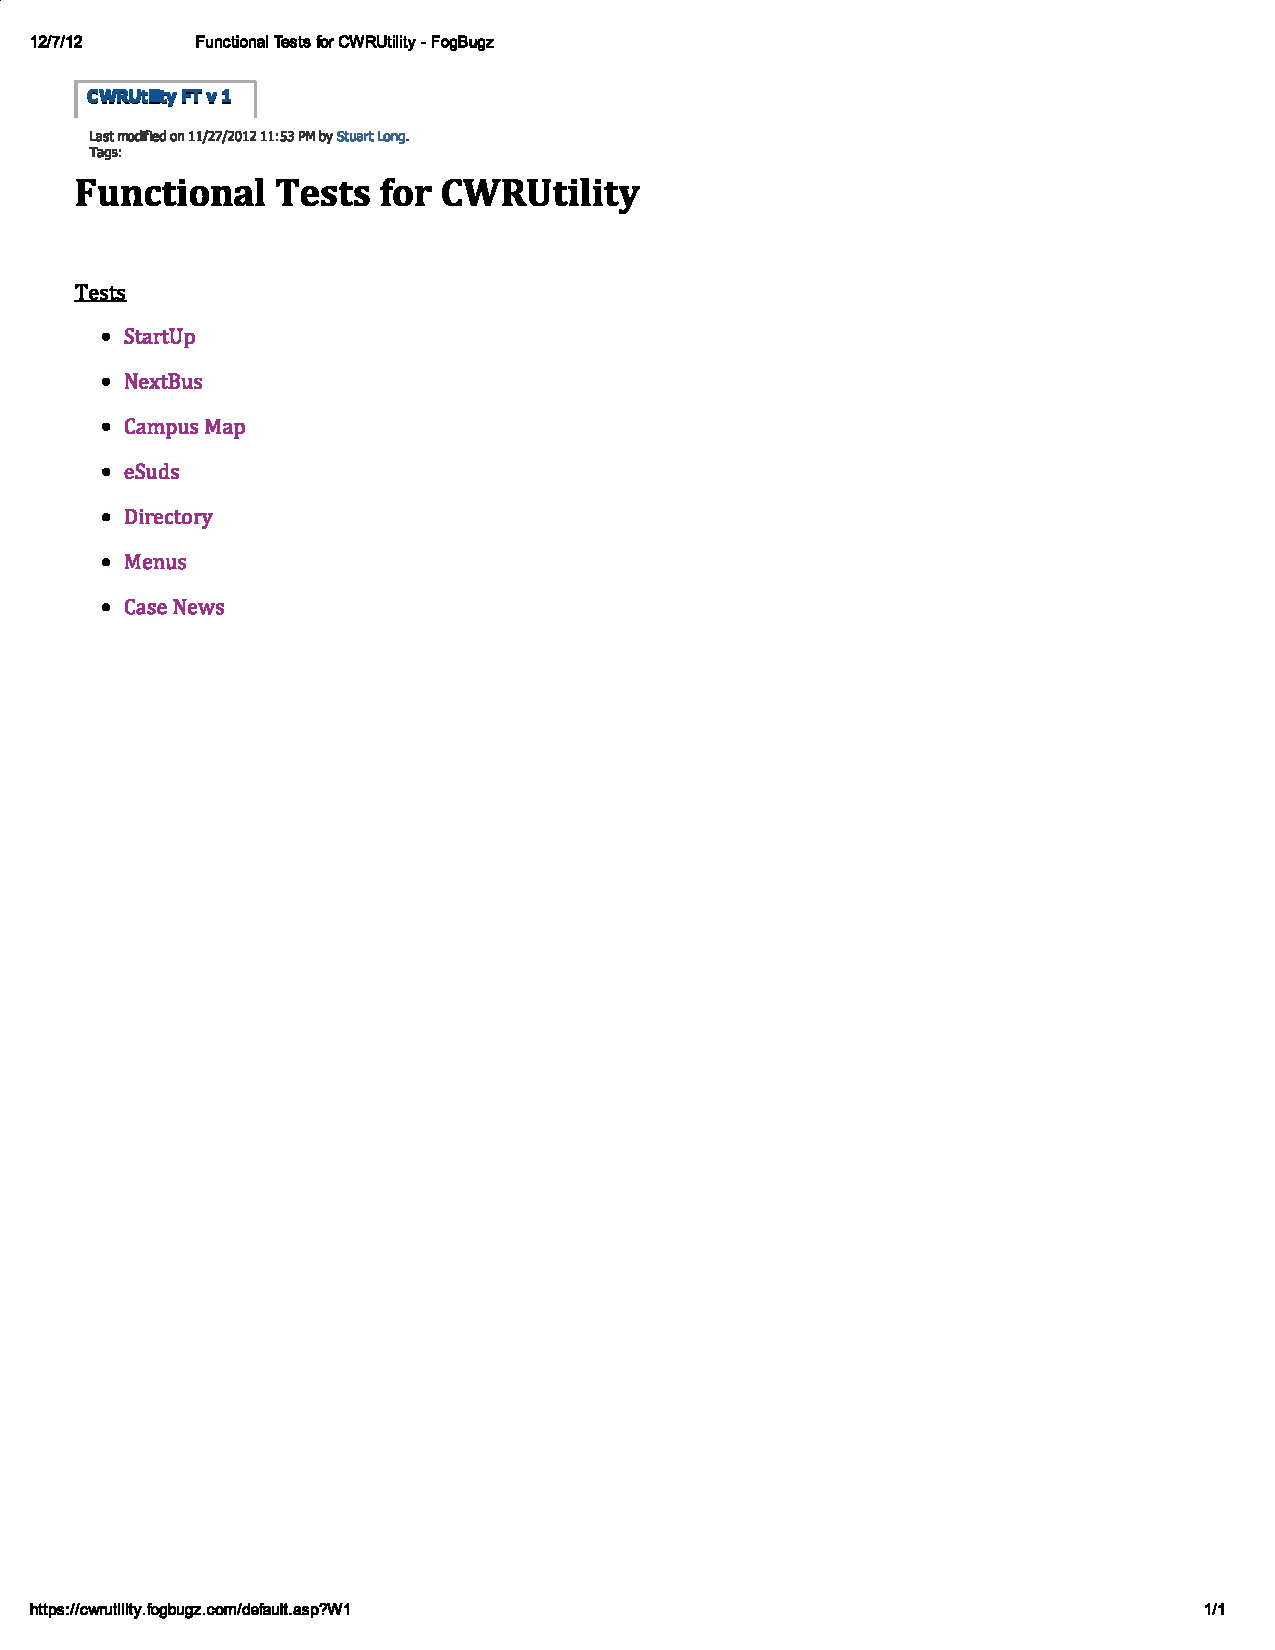
\includepdf[pages={-}]{ftTests.pdf}
\lfoot{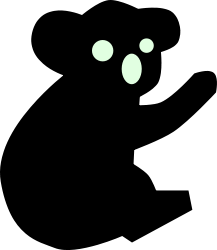
\includegraphics[height=1cm]{DarkKoala.png}}
\end{document}